\documentclass[../../layout.tex]{subfiles}

\begin{document}
\chapter{Método}
\hspace*{3em}Para demonstrar como foi desenvolvido o material técnico e aplicação de valor deste projeto, seguimos por diversas pesquisas e análises de como chegar à um desenvolvimento onde fosse viável sua execução, aplicação e escalabilidade, para que tenha necessidade futura de seu contínuo uso.
\section{Levantamento Bibliográfico}
\hspace*{3em}A aplicação do projeto de forma adequada, levou à muitas buscas teóricas e estudos variados da maneira que pode ser avaliada e aplicada às diversas tecnologias e ferramentas. \par
Dentre elas, podemos citar as mais importantes considerações levadas:

\begin{enumerate}[label=\alph*)]
\itemsep0em
    \item levantamento de requisitos;
    \item linguagem de programação;
    \item ferramentas tenológicas para auxiliar o desenvolvimento e organização do projeto;
    \item casos de uso;
    \item aplicações reais com objetivos similares;
    \item aplicações com as mesmas \emph{frameworks} utilizadas no projeto;
    \item viabilidade.
\end{enumerate}

\subsection{Levantamento de Requisitos}
\hspace*{3em}Foco em analisar quais objetivos queremos chegar e por qual método iremos realizar isso. A intenção era utilizar um microprocessador, escolhido o Raspberry pela sua facilidade de acesso e quantidade de informações de diversos usuários e desenvolvedores, para controlar dispositivos pela internet através de uma maneira simples e otimizada, seja celular ou computador.
\subsection{Linguagem de Programação}
\hspace*{3em}Como existem diversas linguagens de programação, foram realizadas análises variadas das mesmas para entender qual o melhor uso e como se encaixam à essa aplicação que escolhemos. Dentre as muitas, optamos por selecionar linguagens que possuem boa interação com o \emph{frontend} e o \emph{backend}, mantendo um bom desempenho e com um visual prático para o desenvolvimento.
\subsection{Ferramentas Tenológicas}
\hspace*{3em}Ferramentas são necessárias para auxiliar no desenvolvimento, sejam anotações em um tablet, dispositivos auxiliares para realizar análizes ou medições, que não fazem parte exatamente do projeto final, mas tem um grande envolvimento com o mesmo.
\subsection{Casos de Uso}
\hspace*{3em}Empresas focam em atendenter a necessidade de seus clientes de uma forma em que eles saiam satisfeitos e recomendem o serviço, produto ou suporte. Isso faz com que muitas soluções sejam críticamente pensadas e desenvolvidas. Para validação do uso do Elixir, pesquisamos grandes empresas que utilizam essa linguagem em seu \emph{background} \acite{usecases} e encontramos soluções como as seguintes:
\begin{enumerate}[label=\alph*)]
\itemsep0em
    \item Pinterest, uma rede social com 200 milhões de usuários ativos, utiliza Elixir para gerenciar rotas de eventos no sistema;
    \item Financial Times, um jornal eletrônico inglês, utiliza Elixir como ferramenta de meta-programação para criar os DSLs (domínio de linguagens específicas);
    \item Toyota Connected, um serviço de conexão veícular, utiliza Elixir para enviar eventos em tempo real para a central, sobre o trânsito e comportamento do motorista;
    \item SquareEnix, uma grande desenvolvedora de jogos, utiliza Elixir para autenticar jogadores online e comunicação durante o  jogo;
    \item PepsiCo, empresa americana de alimentos, utiliza o Elixir para manter sua ferramenta de comércio virtual ativa.
\end{enumerate}

Com base em todas as empresas analisadas e seus exemplos citados, o uso no Elixir ficou mais claro e objetivo. \par

\subsection{Aplicações Reais}
\hspace*{3em}Pesquisas com aplicações IoT foram realizadas, em que muitas delas utilizam Elixir como base da linguagem e um microprocessador principal, o Rasberry Pi e um microprocessador auxiliar, no caso, um Arduino UNO \acite{elixirunorasp}, para fazer uma comunicação via WEB. Provando que aplicações com Elixir e Raspberry são utilizadas e aplicadas.
\section{Modelo de desenvolvimento}
\hspace*{3em}Existem vários modelos de desenvolvimento que seguem um padrão no momento de criação de negócios, dentre eles podemos citar o Agile, Scrum e Kanban. Cada um desses com seus objetivos e vantagens. Neste projeto focamos em utilizar o modelo Agile, na qual foca em entregar valor através de um \emph{software} que funciona em todos seus quesitos, do que documentações vastas e diversas sobre todas as ações tomadas, execuções detalhadas e implementações sucedidas, porém, não deixa de documentar fatos mais importantes, fazendo com que a análise, teste, desenvolvimento e \emph{design} sejam realizados em paralelo. Na Figura \ref{fig:agile} temos uma demonstração do método citado.

\begin{figure}[H]
\centering
\caption{Método Agile}
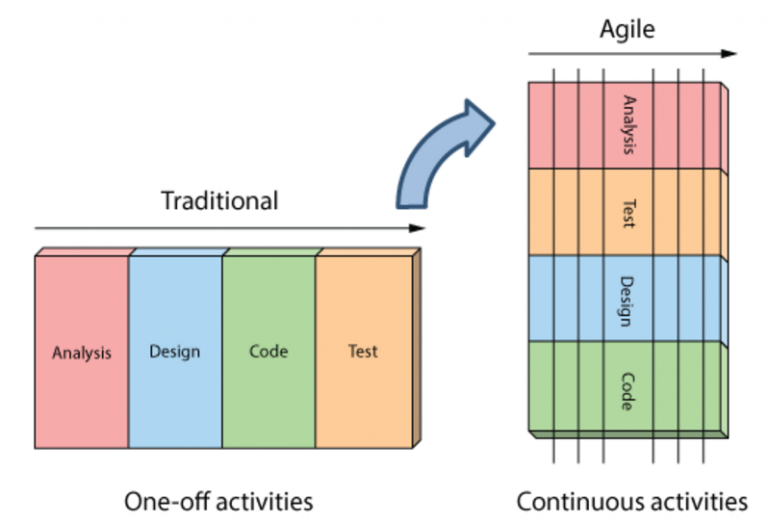
\includegraphics[width=1\textwidth]{assets/static/img/agile.jpg}
\label{fig:agile}

\begin{minipage}{0.5\textwidth}
\raggedright \footnotesize Fonte: Retirado de \acite{agile}
\end{minipage}
\end{figure}

\hspace*{3em}O Kanban, o outro método baseado, trata de um quadro onde colunas de tarefas a ser realizadas, sendo realizadas e já realizadas, são preenchidas com atividades e ao longo de seu desenvolvimento vamos movendo essas tarefas para demonstrar que está ocorrendo evolução. O intuito é que a equipe de desenvolvimento mova essas tarefas assim que cumpridas, de acordo com o perfil e prazo de cada atividade, facilitando a visualização do andamento geral do desenvolvimento. \par
\hspace*{3em}Existem diversas ferramentas com esse intuito, sendo a que escolhemos para nosso projeto o Trello.

\section{Trello}
\hspace*{3em}Trello é um ferramenta onde é possível gerenciar projetos com anotações e cartões, com visual intuitivo e simples manuseio. O objetivo de seu uso é facilitar o desenvolvimento em partes deste projeto e que sejam compartilhadas as conclusões com o time envolvido. Para o Trello utilizamos uma adaptação do método Kanban para realizar as atividades.
\hspace*{3em}Na Figura \ref{fig:trello} temos um exemplo do visual do Trello durante o desenvolvimento:

\begin{figure}[H]
\centering
\caption{Ferramenta Trello}
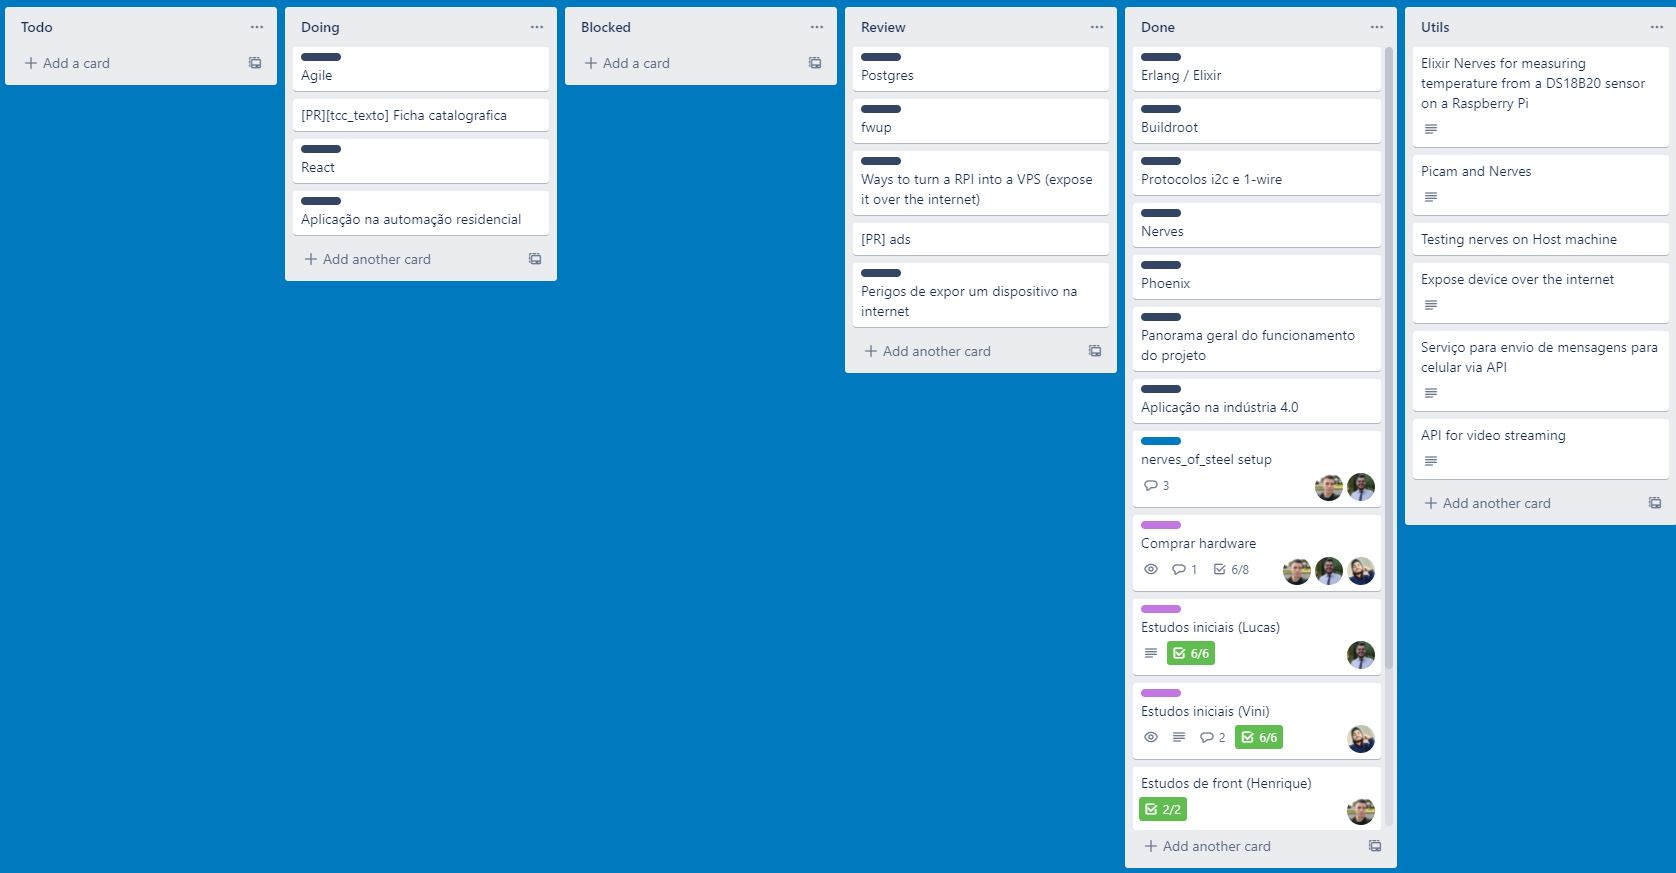
\includegraphics[width=1\textwidth]{assets/static/img/trello.jpg}
\label{fig:trello}

\begin{minipage}{0.5\textwidth}
\raggedright \footnotesize Fonte: autor 
\end{minipage}
\end{figure}

\section{Feature Map}
\hspace*{3em}Para aprofundar em nossos objetivos de projeto, analisamos quais seriam os objetivos finais dos nossos usuários, com isso utilizamos ferramentas em que podemos traçar as necessidades de clientes e suas estórias (\emph{User Stories}) de forma adequada para cada característica (\emph{Feature}). O Feature Map auxilia na visualização dessas características de como caminhar no desenvolvimento com foco em alcançar os objetivos dos usuários finais.

\section{GitHub}
\hspace*{3em}Para ferramenta auxiliar de gerenciamento de códigos optamos pelo GitHub, na qual tem o intuito de realizar a hospedagem de código fonte, arquivos com controle de versão e integração com várias ferramentas e ambientes. Nele podemos realizar alterações no código em tempo real e acomapnhar todas essas modificações de uma maneira integrada. No projeto criamos 3 repositórios:

\begin{enumerate}[label=\alph*)]
\itemsep0em
    \item nerves of steel, onde hospedamos nosso código \emph{backend};
    \item paralysis, onde hospedamos nosso código \emph{frontend};
    \item tcc texto, onde hospedamos nossa dissertação e documentação do tcc.
\end{enumerate}

\begin{figure}[H]
\centering
\caption{Ferramenta GitHub}
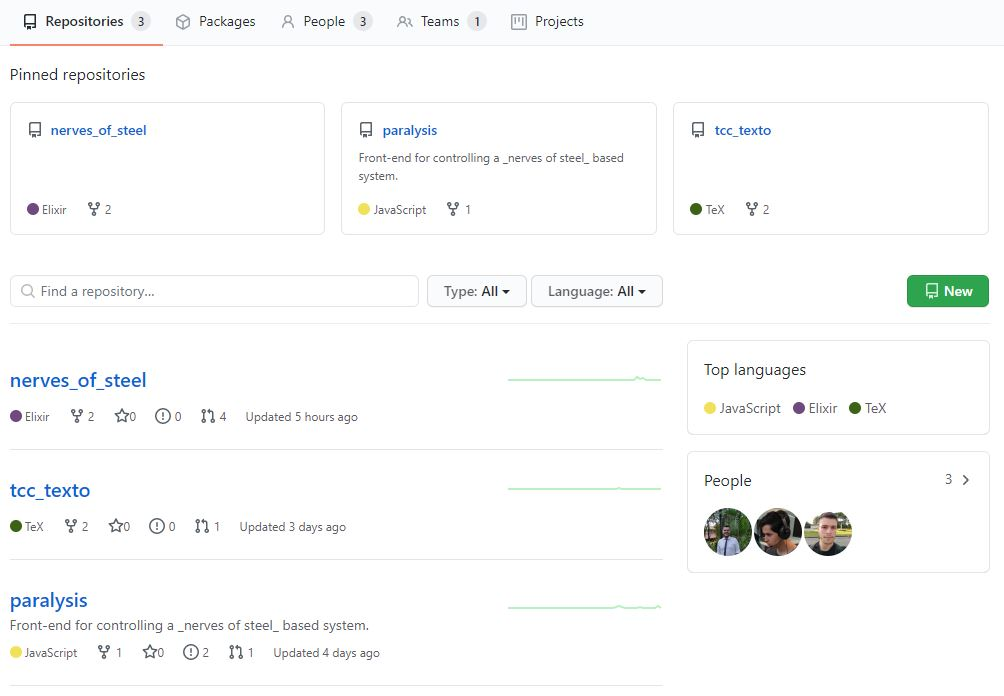
\includegraphics[width=1\textwidth]{assets/static/img/git.jpg}
\label{fig:i2c_structure}

\begin{minipage}{0.5\textwidth}
\raggedright \footnotesize Fonte: autor 
\end{minipage}
\end{figure}


\section{Aplicação com Nerves}
\hspace*{3em}\blindtext[1]
\section{Phoenix}
\hspace*{3em}\blindtext[1]
\section{Aplicação Ecto}
\hspace*{3em}\blindtext[1]
\section{Aprendizado React e Desenvolvimento}
\blindtext
\end{document}
